\chapter{Proposed Work}
Image enhancement improves the quality of images for human viewing. There are often serious discrepancies existing between images and the direct observation of the real scenes. Human perception has natures of dynamic range compression and color rendition on the scenes. It can compute the details across a large range of spectral and lightness variations, thus it is color constant. Single-scale Retinex (SSR) was defined as an implementation of center/surround Retinex. Superposition of weighted different scale SSR balances both dynamic range compression and tonal rendition, which is Multiscale Retinex (MSR). For color images, spatial averages of the three color bands are far from equal, thus the output appears grey. To address this issue, a weight factor for different channels is introduced which is Multiscale Retinex with color restoration (MSRCR). In this paper, SSR, MSR and MSRCR systems for image enhancement are implemented and their performances are compared using MATLAB as the software tool.

\section{Introduction}
The human visual system is better than machines when processing images. Observed images of a real scene are processed based on brightness variations. The images captured by machines are easily affected by environmental lighting condition, which tends to reduce its dynamic range[1]. On the contrary, the human visual system can automatically compensate the image information by psychological mechanism of color constancy[2]. Color constancy, an approximation process of human perception system, makes the perceived color of a scene or objects remain relatively constant even with varying illumination conditions. Land [3] proposed a concept of the Retinex, formed from "retina" and "cortex", suggesting that both the eye and the brain are involved, to explain the color constancy processing of human visual systems. Although single-scale retinex (SSR) algorithm could support different dynamic-range compressions, the multi-scale retinex (MSR) can better approximate human visual processing by transforming recorded images into a rendering which is much closer to the human perception[4] of the original scene. MSR is good for gray images. But it could be a problem for the color images because it does not consider the relative intensity of color bands. This can be seen from MSR output which is the relative reflectance‘s[5] in the spatial domain. Considering the images out of gray world, whose average intensity for the three color bands are far from equal, the output pixel values of MSR for three channels will be more close, which makes it look more gray.The solution to this problem is MSRCR that introduces weights for three color channels depending on the relative intensity of the three channels in the original images


\section{Retinex in Image Processing}
Land described that the fundamental challenge of color vision shifted to the ability to predict lightness; that is, the spatial interactions found in post-receptor neural processes. In 1967 Land and McCann proposed a computational model for calculating lightness from the array of all scene radiances. The model compared each pixel with every other pixel in an image. The goal was to calculate the sensation of image segments that equaled what observers saw. In the past 50 years, there have been many implementations and variations of this process. They are called Retinex algorithms. It is curious that Land reserved the use of the term “Retinex” to describe three independent lightness channels. Today’s usage of the word includes a much wider range of computer algorithms that build calculated appearances out of arrays of radiances. To calculate lightnesses in complex scenes, one must: Capture scene radiances, Convert scene radiances to cone and rod quanta catches, Calculate lightness using all pixels in the scene, Compare calculated lightness with observer matches. The Land and McCann model used: Edge ratios, Gradient threshold (found to be unnecessary in later studies), Multiplication of edge ratios (made long-distance interactions), Reset to maxima (scaled the output) (introduced dependence on scene content, e.g., simultaneous contrast) Average of many spatial comparisons. The first computer implementation of the model used an array of 20 by 24 pixels. McCann, McKee, and Taylor showed that long-, middle-, and short-wave computed lightnesses predicted observer matches of color Mondrian’s in color constancy experiments.

Since the late 1960s, computer imaging has shown remarkable advances. Digital images have replaced film in most of photography. Computer graphics has made image synthesis ubiquitous. Retinex image processing has grown with the advances in digital imaging . In the early 1980s Frankle and McCann introduced a multi-resolution algorithm that allowed efficient comparison of all pixels in the image. Jobson and Kotera with their colleagues have studied the NASA Retinex. Rizzi and colleagues have developed the Milan Retinex. Sobol extended that Retinex algorithm was used in the design of commercial cameras. Other algorithms have used Retinex spatial processing in color gamut-mapping applications.

The important feature of real complex scenes is that the illumination is rarely uniform. Shadows and multiple reflections increase the dynamic range of light coming to our eyes and to cameras. The application of Retinex algorithms to high dynamic range (HDR) scenes has become a major topic of research and engineering applications. The limits of HDR scene capture and reproduction are controlled by optics, namely, optical veiling glare. Camera glare limits the range of light on the sensor, just as intraocular glare limits the range of light on the retina. The scene content controls the range of light in images. Vision’s post-receptor neural processes compensate for veiling glare. That explains humans’ high dynamic range of appearances from low-dynamic-range retinal images. The spatial mechanisms modeled by Retinex algorithms play a major role in compensating for glare and generating our range of color and lightness sensations.

Over the years many variations of spatial processing mimicking human vision have been called Retinex algorithms.[2]

The different types of retinex algorithms are: 
\begin{itemize}
		\item Single Scale Retinex algorithm (SSR)
		\item Multiscale Retinex algorithm (MSR)
		\item Multiscale retinex with Color Restoration algorithm (MSRCR) 
\end{itemize}
	
\subsection{Single Scale Retinex (SSR)}
The basics of SSR include a logarithmic photoreceptor function that approximates the vision system based on a center/surround [6] function. The SSR is given by:
\begin{equation}
	R_{i}(x,y)=\log_{i}-\log[F(x,y)\*I_{i}(x,y)]
\end{equation}
where $I_{i} (x,y)$ is image distribution in the ith color band,$F(x,y)$ is the normalized surround function[7] such that:

\begin{equation}
	\iint F(x,y)dxdy=1
\end{equation}

The purpose of the logarithmic manipulation is to transform a ratio at the pixel level to a mean value for a
larger region. The general form of the center/surround retinex is similar to the Difference-of-Gaussian (DOG)
function widely used in natural vision science to model both the receptive fields of individual neurons and
perceptual processes. The only extensions required are i) to greatly enlarge and weaken the surround Gaussian (as
determined by its space and amplitude constants) and ii)to include a logarithmic function to make subtractive
inhibition into a shunting inhibition (i.e., arithmetic division). The surround space function computes the
average of the surrounding pixel values and assigns it to the center pixel.
Land [3] proposed an inverse square spatial surround function:

\begin{equation}
	F(x,y)=K*exp(-\frac{r^2}{c^2})
\end{equation}
Moore suggested the exponential formula with absolute
parameter:

\begin{equation}
	F(x,y)=exp(-\frac{r}{c}
\end{equation}
Hurlbert [8] suggested:

\begin{equation}
	F(x,y)=K*exp(-\frac{r^2}{c^2}
\end{equation}

For a given space constant, the inverse-square surround
function accounted for a greater response from the
neighboring pixels than the exponential and Gaussian
functions. The spatial response of the exponential
surround function was larger than that of the Gaussian
function at distant pixels. Therefore, the inverse-square
surround function was more commonly used in global
dynamic range compression and the Gaussian surround
function was generally used in regional dynamic range
compression[9]. The exponential and Gaussian surround
functions were able to produce good dynamic range
compression over neighboring pixels. The selection of
space constant is related with visual angle in the direct
observation. But the value cannot be theoretically
modeled and determined. Basically there is a trade-off
between dynamic compression, (for example, details in
the shadow) and color rendition.
SSR is incapable of simultaneously providing sufficient
dynamic range compression and tonal rendition. It also
introduces halos around the objects.

\subsection{Multiscale Retinex (MSR)}
In order to preserve both the dynamic range compression
and color rendition, Multi-scale retinex, which is a
combination of weighted different scales of SSR [10], is
a good solution:

\begin{equation}
	R_{MSR_{i}}=\sum_{n=1}^{N}w_{n}R_{n_{i}}
\end{equation}

where N is the number of the scales, Rni is the ith
component of the nth scale, wn is the weight of the nth
scale. For MSR, the number of scales needed, scale
values and weight values are important. Experiments
showed that three scales are enough for most of the
images and the weights can be equal. Generally fixed
scales of 15, 80 and 250 can be used, or scales of fixed
portion of image size can be used. The weights can be
adjusted to weigh more on dynamic range compression
or color rendition [11]. The MSR based images have
significant dynamic range compression in the boundary
between the light parts and dark parts and reasonable
color rendition in the whole image scale.

MSR combined various SSR weightings, selecting the
number of scales used for the application and evaluating
the number of scales that can be merged. Important
issues to be concerned were the number of scales and
scaling values in the surround function, and the weights
in the MSR. The best weights had to be chosen in order
to obtain suitable dynamic-range compression at the
boundary between light and dark parts of the image, and
to maximize the brightness rendition [12] over the entire
image. MSR worked by compensating for lighting
variations to approximate the human perception of a real
scene. There were two methods to achieve this: (1)
compare the psychophysical mechanisms between the
human visual perceptions of a real scene and a captured
image, and (2) compare the captured image with the
measured reflectance values of the real scene.

Thus the method involved combining specific features of
MSR with processes of SSR, in which the
center/surround operation was a Gaussian function. The
logarithm was then applied after surround function
processing (i.e., two-dimensional spatial convolution).
Next, appropriate gain and offset values were determined according to the retinex output and the characteristics of
the histogram. These values were constant for all the
images. This procedure yielded the MSR function.
However, it is difficult to predict whether the color of the
reproduction will be accurate; and it has issues of color
sensitivity [13].



\subsection{Multiscale retinex with Color Restoration algorithm (MSRCR)}
To address the drawback of MSR with regard to color
restoration, we introduced weights for three color
channels depending on the relative intensity of the three
channels in the original images. The relative intensity of
three channels is given by:

\begin{equation}
	I_{i}(x,y)=\frac{I_{i}(x,y)}{\sum_{j=1}^{s}I_{i}(x,y)}
\end{equation}

$I_{i}$ is the $i^{th}$ band of the input image and S is the total
number of color bands. The color restoration [14] is
given by:

\begin{equation}
	C_{i}(x,y)=f[I_{i}(x,y)]
\end{equation}

The best overall color restoration function is given by:

\begin{equation}
	C_{i}(x,y)=\beta \log[\alpha I_{i}(x,y)]
\end{equation}

where $\beta$ is the gain constant and $\alpha$ controls the strength of
non-linearity.
The general form of the MSRCR can be summarized by
the following equation:

\begin{equation}
	I_{i}(x,y_=\frac{d_{max}}{r_{max}-r_{min}}*(I_{i}(x,y)-r_{min})
\end{equation}

where $i =1, ….. N$, ws is the weight of the scale, $I_{i}$ is the
ith band of the input image, and N is the number of bands
in the input image. The surround function $M_{s}$ is defined
by:

\begin{equation}
	M_{s}(x,y)=K exp[{\sigma^{2}}_{s}/(x^{2}+y^{2})]
\end{equation}

where $\sigma_{s}$ is the standard deviation of the $S^{th}$ surround
function, and

\begin{equation}
	\iint K exp[{\sigma^{2}}_{s}/(x^{2}+y^{2})]dx dy =1
\end{equation}

\begin{equation}
	F_{i}(x,y)=G_{f} \log big[\frac{I_{i}(x,y)}{\sum_{n=1}^N I_{n}(x,y)}-O_{f}\big]
\end{equation}

The $G_{f}$ and Of are color restoration factors defined as
gain and offset respectively. The final gain and offset
values are needed to scale the output of the $\log$ domain
operations to the (R, G, B) color space, and $G_{f}$ and Of
control the degree to which the color restoration function
$F(x,y)$ affects the overall color of the output image. These
constants, the number of scales, $S$, and the widths of the
surround functions $\gamma_{s}$, are image independent in the sense
that we apply the same (canonical) set of constants to
every image that we process.

Some of the images processing related issues in MSRCR
are:
\begin{itemize}
	\item Negative Offset:\\
	This is an attempt to increase the dynamic range (i.e.
visual contrast) provided by the device but is often
photometrically incorrect and results in false zeroes. The
effect of the MSRCR is to produce a harsher-than-normal
contrast. A simple correction, i.e. application of a
positive offset to the original image can mitigate this
effect.

\end{itemize}

\begin{itemize}
	\item Automatic Gain and Offset [15]:\\
	A negative offset is typically applied to map the
minimum value to black and then a gain is applied to
map the resultant maximum value to white. Care is taken
to ensure that actual white exists in the scene. The
MSRCR is very resilient to such adjustments. Since the
difference between the MSRCR outputs in the original
and the auto/gain case is insignificant, the result is not
shown here.

\end{itemize}

\begin{itemize}
	\item Positive Offset:\\
	Typically brightness in an image is increased by applying
a positive offset, which often manifests itself as an
overall haziness in the input image. Though the
application of the MSRCR reduces this haziness, there is
still a sense of haziness overall. Further alleviation of this
effect can be achieved by reducing the final offset value;
$O_{r}$ from its canonical value.
In this paper, color problems were focused utilizing
MSRCR as an image processing technique to solve the
problems of the accuracy of the color of the reproduction.
The main practical consequence of MSR is that it is not
appropriate for applications which are sensitive to color.
The results of MSRCR prove that it is efficient to avoid
graying out effects. It maintains good color rendition and
color constancy.
\end{itemize}

\begin{figure}
	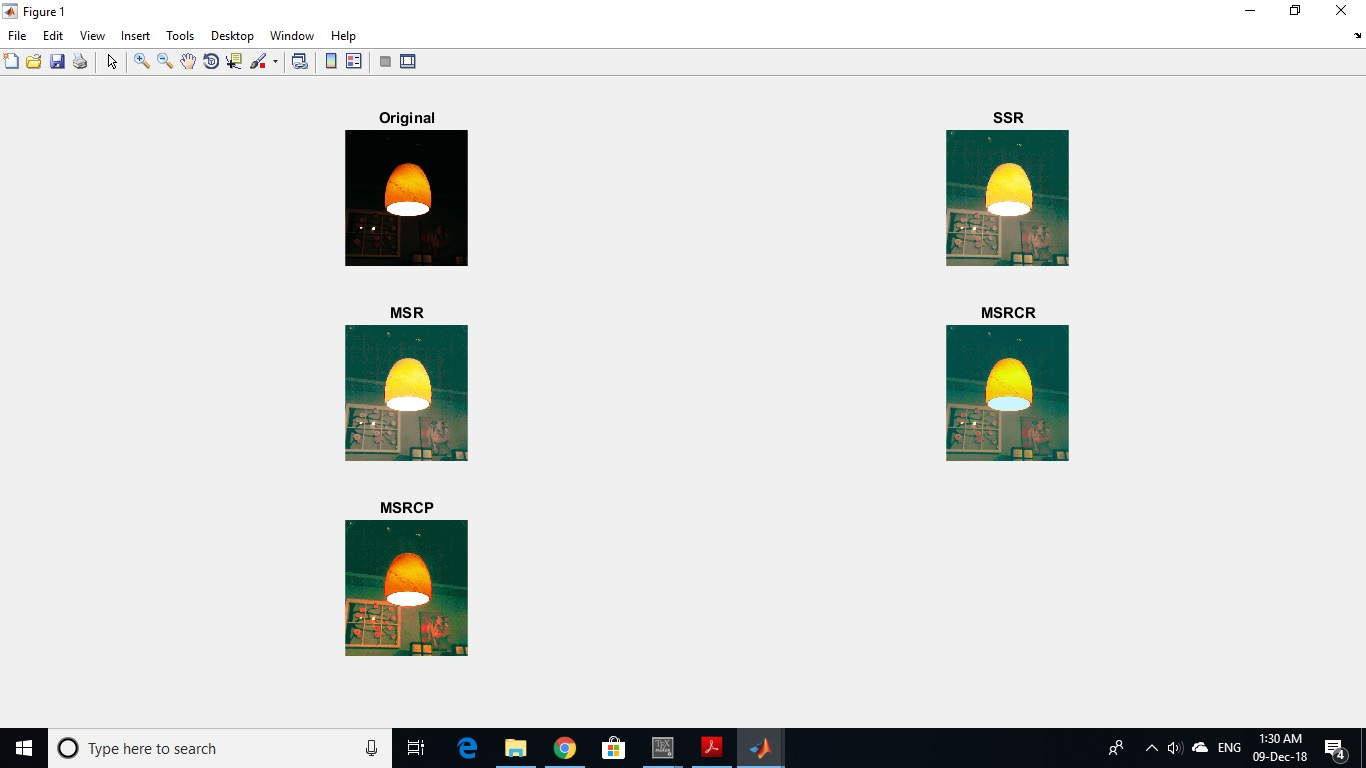
\includegraphics[scale=0.5]{images/ch3/retinexModel.jpg}
	\caption{Result of Retinex Model}
\end{figure}

\section{Power Law Transformation}
Image enhancement can be carried out in the spatial or the Fourier domains and one of the important
parameters to be looked at in this context is contrast enhancement. In the spatial domain,
the methods used may be further classified into: gray level transformations, histogram processing,
etc. As mentioned above, histogram equalization suffers from the fact that it may sometimes
decrease the contrast. Histogram specification or matching can be tailor-made to suit the images
but requires lot of user input. Similarly, power law transformations or piece-wise linear transformation
functions also require lot of user input. In the former case one has to choose the exponent
appearing in the transformation function, while in the latter case one has to choose the slopes
and ranges of the straight lines which form the transformation function.

The power-law transformation is usually defined as

\begin{equation}
	s=c \thinspace r^\gamma
\end{equation}
where $s$ and $r$ are the gray levels of the pixels in the output and the input images, respectively and
$c$ is a constant. These power law transformation functions are shown graphically in the diagram
(figure \ref{fig:powerLawTransformation}).
Figure \ref{fig:powerLawTransformation} shows the plot of power law transformation with the input gray level $r$ along the $x$ axis and the output gray level $s$ on the $y$ axis for various values of $\gamma$ .
We will now consider that these transformations are applied on a low contrast image. We
assume that the background and foreground peaks have almost merged together in such a low
contrast image. Let $r_{max}$ be the dominant peak in the histogram. If $r_{max}$ has a large value (in the
range $150\textrm{--}255$), then it is seen from the above graph that contrast stretching occurs by choosing
$\gamma \textgreater 1$ whereas for dark images ($r_{max}$ lies in the range $0\textrm{--}100$), we see that choosing $\gamma \textless 1$ leads
to contrast stretching. We can of course, automate this procedure for choosing the appropriate
exponent, by finding out the peak value in the histogram. However, we can further generalize
this procedure so that the most appropriate value of the exponent is chosen.

\begin{figure}
	\centering
	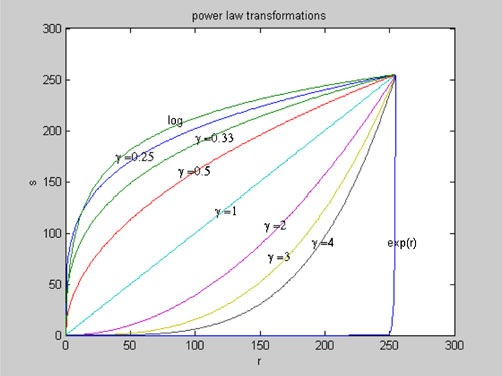
\includegraphics[scale=0.9]{images/ch3/powerLawTransformation.jpg}
	\caption{Plot of power law transformation for various $\gamma$ with input gray level along $X$ axis and output
gray level along $Y$ axis.}
	\label{fig:powerLawTransformation}
\end{figure}

\section{Histogram Equalization}
An image histogram is a type of histogram that acts as a graphical representation of
the tonal distribution in a digital image. It plots the number of pixels for each tonal
value. A histogram is a representation of a frequency distribution. The histogram
of a digital image with $G$ total possible intensity levels in the $[0,G − 1]$ is defined
as the discrete function:

\begin{equation}
	p(\gamma_{k})=\frac{n_{k}}{n}
\end{equation}

Where $\gamma_{k}$ is the intensity level in the original raw image $n_{k}$ is the number of
pixels in the image whose intensity level is n is the total no of pixels.

Histogram equalization is used to enhance the contrast of the image, it spreads the
intensity values over full range. Histogram equalization technique can’t be used for
images suffering from non-uniform illumination in their backgrounds as this process
only adds extra pixels to the light regions of the image and removes extra pixels from
dark regions of the image resulting in a high dynamic range in the output image.The
goal of histogram equalization is to spread out the contrast of a given image evenly
throughout the entire available dynamic range.

\begin{figure}
	\centering
	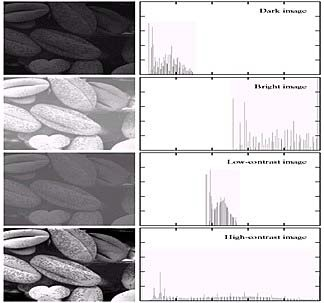
\includegraphics[scale=1]{images/ch3/histogramEqualization.jpg}
	\caption{Seed Image and its histogram}
	\label{fig:histogramEqualization}
\end{figure}

In histogram equalization technique, it is the probability density function (pdf)
that is being manipulated. To make it simple, what histogram equalization technique
does is that, it changes the pdf of a given image into that of a uniform probability
density function that spreads out from the lowest pixel value ($0$ in this case) to
the highest pixel value $(L − 1)$ . This can be achieved quite easily if the pdf is a
continuous function. However, since we are dealing with a digital image, the pdf
will be a discrete function. Lets suppose we have an image $x$ , and let the dynamic
range for the intensity $\gamma_{k}$ varies from $0$ (black) to $L1$ (white). This pdf can be
approximated using the probability based on the histogram $p(\gamma_{k})$ as follow:

\begin{equation}
	pdf(x)=p(\gamma_{k})= \frac{total\;pixels\;with\;intensity\; \gamma_{k}}{total\;pixels\;I\;image\;x}
\end{equation}

From this pdf, we can then obtain the cumulative density function (cdf) as follows:

\begin{equation}
	cdf(x)=\sum_{k=0}^{L-1}p(\gamma_{k})
\end{equation}

Where $p(\gamma_{k})$ is the probability for pixel of intensity. The output of a pixel from
the histogram equalization operation is then equal to the cdf of the image or mathematically :

\begin{equation}
	p(s_{k})=\sum_{k=0}^{L-1}p(\gamma_{k})
\end{equation}

To get the value of the pixel, $p(s_{k})$ needs to be multiplied by $L1$ and then round
it to the nearest integer

\subsection{Equalization on Color Image}
\begin{itemize}
	\item \textbf{Equalize R, G, B components independently (method1)}\\
			This scheme is one of the mostly used methods for color image processing.
			Each channels of RGB space are processed using Histogram Equalization
			independently[2].After the Equalize the R,G,B components we concate all the three
			components and get the better image compare to input image.

			\begin{figure}
				\centering
				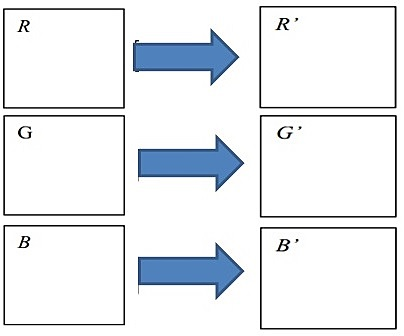
\includegraphics[scale=1]{images/ch3/method1.jpg}
				\caption{Block diagram showing the implementation of Method 1}
				\label{method1}
			\end{figure}
	\item \textbf{Equalize tha V Component from HSV Color Space (method 2)}\\
			In order to process color image in RGB color space using this scheme, image first
			must be transformed to hue, saturation and luminance (HSV) color space.Here	
			Brightness is a synonym of intensity. Hue represents the impression related to the
			dominant wavelength of the color stimulus Saturation shows the relative color purity
			(amount of white light in the color).
			Hue and Saturation taken together are called the chromaticity coordinates (polar
			system).
			In this method we apply the Histogram Equalization on V component on HSV
			color space .After the Equalize the V we combine the V with H and S .Then we get
			the better image compare to input image.\\
			$HSV \rightarrow H, S, V$\\
			$V \rightarrow V(equalize)$\\
			$HSV(equalize) \rightarrow H, S, V(equalize)$\\
	\item \textbf{Equalize the Y Component from YIQ Color Space(method 3)}\\
			In order to process color image in RGB color space using this scheme, the image
			first must be transformed to YIQ color space[4][5].\\
			Here\\
			The Y component represents the luma information, and is the only component used
			by black-and-white television receivers.\\
			I stands for in-phase\\
			Q stands for quadrature\\
			I and Q represent the chrominance information.\\

			In this method we apply the Histogram Equalization on Y component on YIQ
			color space .After the Equalize the Y we combine the Y with I and Q .Then we get the better image compare to 				input image.\\
			$YIQ \rightarrow YIQ$\\
			$Y \rightarrow Y(equalize)$\\
			$YIQ(equalixe) \rightarrow Y, I, Q(equalize)$\\
\end{itemize}

\section{Adaptive Histogram Equalization(AHE) method}
This is an extension to traditional Histogram Equalization
technique. It enhances the contrast of images by transforming
the values in the intensity image I. Unlike HISTEQ, it operates
on small data regions (tiles), rather than the entire image. Each
tile's contrast is enhanced, so that the histogram of the output
region approximately matches the specified histogram. The
neighboring tiles are then combined using bilinear interpolation
in order to eliminate artificially induced boundaries.
The contrast, especially in homogeneous areas, can be limited
in order to avoid amplifying the noise which might be present
in the image.
\begin{itemize}
	\item Algorithm Steps:
	\begin{enumerate}
		\item Obtain all the inputs: Image, Number of regions in row and column directions, Number of bins for the 	
		histograms used in building image transform function (dynamic range), Clip limit for contrast limiting (normalized 	
		from 0 to 1)
		\item Pre-process the inputs: Determine real clip limit from the normalized value if necessary, pad the image 
		before splitting it into regions
		\item Process each contextual region (tile) thus producing gray level mappings: Extract a single image region, make 
		a histogram for this region using the specified number of bins, clip the histogram using clip limit, create a 
		mapping (transformation function) for this region.
		\item Interpolate gray level mappings in order to assemble final CLAHE image: Extract cluster of four neighbouring 
		mapping functions, process image region partly overlapping each of the mapping tiles, extract a single pixel, apply
		four mappings to that pixel, and interpolate between the results to obtain the output pixel; repeat over the entire 
		image.
	\end{enumerate}
\end{itemize}

In low contrast images, the features of interest may occupy only a
relatively narrow range of gray scale, with the majority of gray levels occupied by
“uninteresting areas” such as background and noise. These “uninteresting areas”
may also generate large counts of pixels and hence, large peaks in the
histogram. In this case, the global histogram equalization amplifies the image
noise and increases visual graininess or patchiness. The global histogram
equalization technique does not adapt to local contrast requirements, and minor
contrast differences can be entirely missed when the number of pixels falling in a
particular gray range is small.

Adaptive Histogram Equalization (AHE) is a modified histogram
equalization procedure that optimizes contrast enhancement based on local
image data. The basic idea behind the scheme is to divide the image into a grid
of rectangular contextual regions, and to apply a standard histogram equalization
in each. The optimal number of contextual regions and the size of the regions
depend on the type of input image, and the most commonly used region size is
8x8 (pixels). In addition, a bi-linear interpolation scheme is used to avoid
discontinuity issues at the region boundaries.

Figure \ref{fig:bilinearInterpolation} illustrates the application of the interpolation scheme at the
boundaries. Gray level assignment at the sample positions indicated by the white
dot are derived from gray-value distributions in the surrounding contextual regions. The points A, B, C, and D are the centers of the surrounding contextual
regions; region-specific gray level mappings (gA(s), gB(s), gC(s) and gD(s)) are
based on the histogram equalization of the pixels contained. Thus, assuming that
the original pixel intensity at the sample point is s, its new gray value s’ is
calculated by bilinear interpolation of the gray-level mappings that were
calculated for each of the surrounding contextual regions:

\begin{equation}
	s'=(1-y)((1-x)g_{A}(s) + xg_{B}(s))+y(((1-x)g_{c}(s)+xg_{D}(s))
\end{equation}

where x and y are normalized distances with respect to the point A. This
gray level interpolation is repeated over the entire image

\begin{figure}
	\centering
	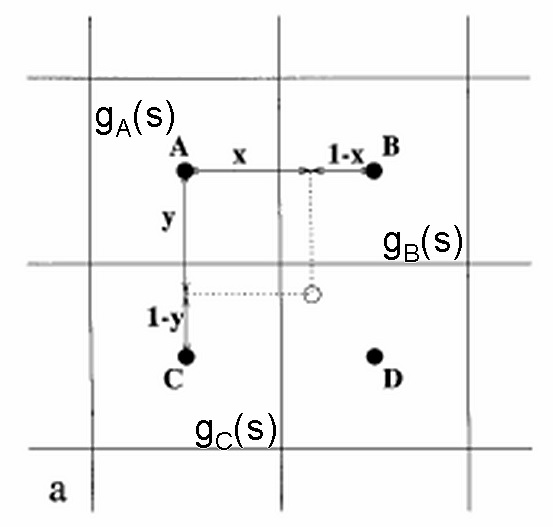
\includegraphics[scale=0.7]{images/ch3/bilinearInterpolation.jpg}
	\caption{Bilinear interpolation to eliminate region boundaries[From Zuiderveld, 1994].}
	\label{fig:bilinearInterpolation}
\end{figure}

AHE is able to overcome the limitations of the standard equalization
method as discussed earlier, and achieves a better presentation of information
present in the image. However, AHE is unable to distinguish between noise and
features in the local contextual regions. Hence, background noise is amplified in
“flat” or “featureless” regions of the image, which is a major drawback of the
method.

\subsection{Contrast Limited Adaptive Histogram Equalization (CLAHE)}
The noise problem associated with AHE can be reduced by limiting
contrast enhancement specifically in homogeneous areas. These areas can be
characterized by a high peak in the histogram associated with the contextual
regions since many pixels fall inside the same gray level range. The Contrast
Limited Adaptive Histogram Equalization (CLAHE) limits the slope associated
with the gray level assignment scheme to prevent saturation, as illustrated in
Figure \ref{CLAHE}. This process is accomplished by allowing only a maximum number of
pixels in each of the bins associated with the local histograms. After “clipping” the
histogram, the clipped pixels are equally redistributed over the whole histogram
to keep the total histogram count identical
\begin{figure}
	\centering
	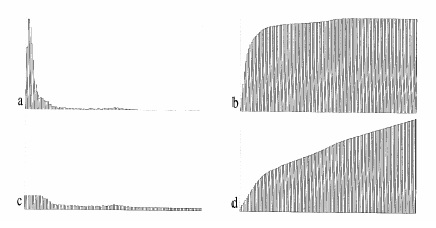
\includegraphics[scale=1]{images/ch3/CLAHE.jpg}
	\caption{Principle of contrast limiting as used in CLAHE. (a)
Histogram of a contextual region containing many background pixels.
(b) Calculated cumulative histogram. (c) Clipped histogram with excess
pixels redistributed throughout the histogram. (d) Cumulative clipped
histogram with maximum slope set to the clip limit [From Zuiderveld,
1994].}
\label{CLAHE}
\end{figure}

The clip limit is defined as a multiple of the average histogram contents
and is actually a contrast factor. Setting a very high clip limit basically limits the clipping and the process becomes a standard AHE technique. A clip or contrast
factor of one prohibits any contrast enhancement, preserving the original image.
The main advantages of the CLAHE transform are its modest
computational requirements, ease of use and excellent results on most images. The CLAHE image has less amplified noise and avoids the brightness saturation in the standard histogram equalization.

CLAHE does have its limitations. Since the method is aimed at optimizing
contrast, there no direct 1-to-1 relationship between the gray values of the
original image and the CLAHE processed result. Pixels of the same gray level in
the original image may be mapped to different gray levels in the output image,
because of the equalization process and bilinear interpolation. Consequently,
CLAHE images are not suited for quantitative measurements that rely on
physical meaning of image intensity [Zuiderveld, 1994].

